As part of a collaborative \textit{Arts, Science and Culture} Grant sponsored by the University of Chicago's Institute for Molecular Engineering, Divisions of the Biological and Physical Sciences, the Humanities, and the Office of the Vice President for Research and for National Laboratories, I undertook a .

\section{The ship of Theseus as a metaphor for life}



{\setstretch{1.0}
\blockquote{ The ship wherein Theseus and the youth of Athens returned from Crete had thirty oars, and was preserved by the Athenians down even to the time of Demetrius Phalereus, for they took away the old planks as they decayed, putting in new and stronger timber in their places, in so much that this ship became a standing example among the philosophers, for the logical question of things that grow; one side holding that the ship remained the same, and the other contending that it was not the same. ---Plutarch's Life of Theseus, as translated by John Dryden }
}

\section{Experiments with plastic filament sculpture}

\begin{figure}[h!]
\centering
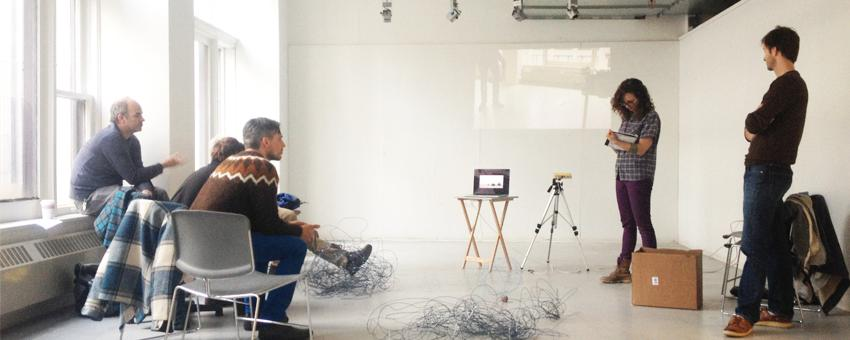
\includegraphics[width=\hsize]{art/collab1.jpg}
\caption{\label{fig:art_2}  }
\end{figure}

\begin{figure}[h!]
\centering
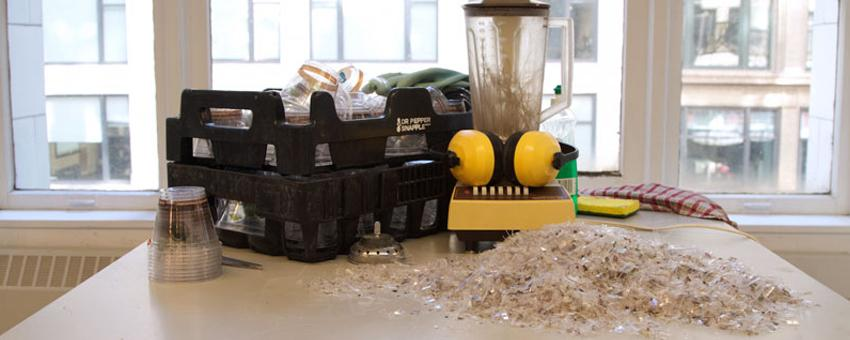
\includegraphics[width=\hsize]{art/shavings.jpg}
\caption{\label{fig:art_1}  }
\end{figure}

\begin{figure}[h!]
\centering
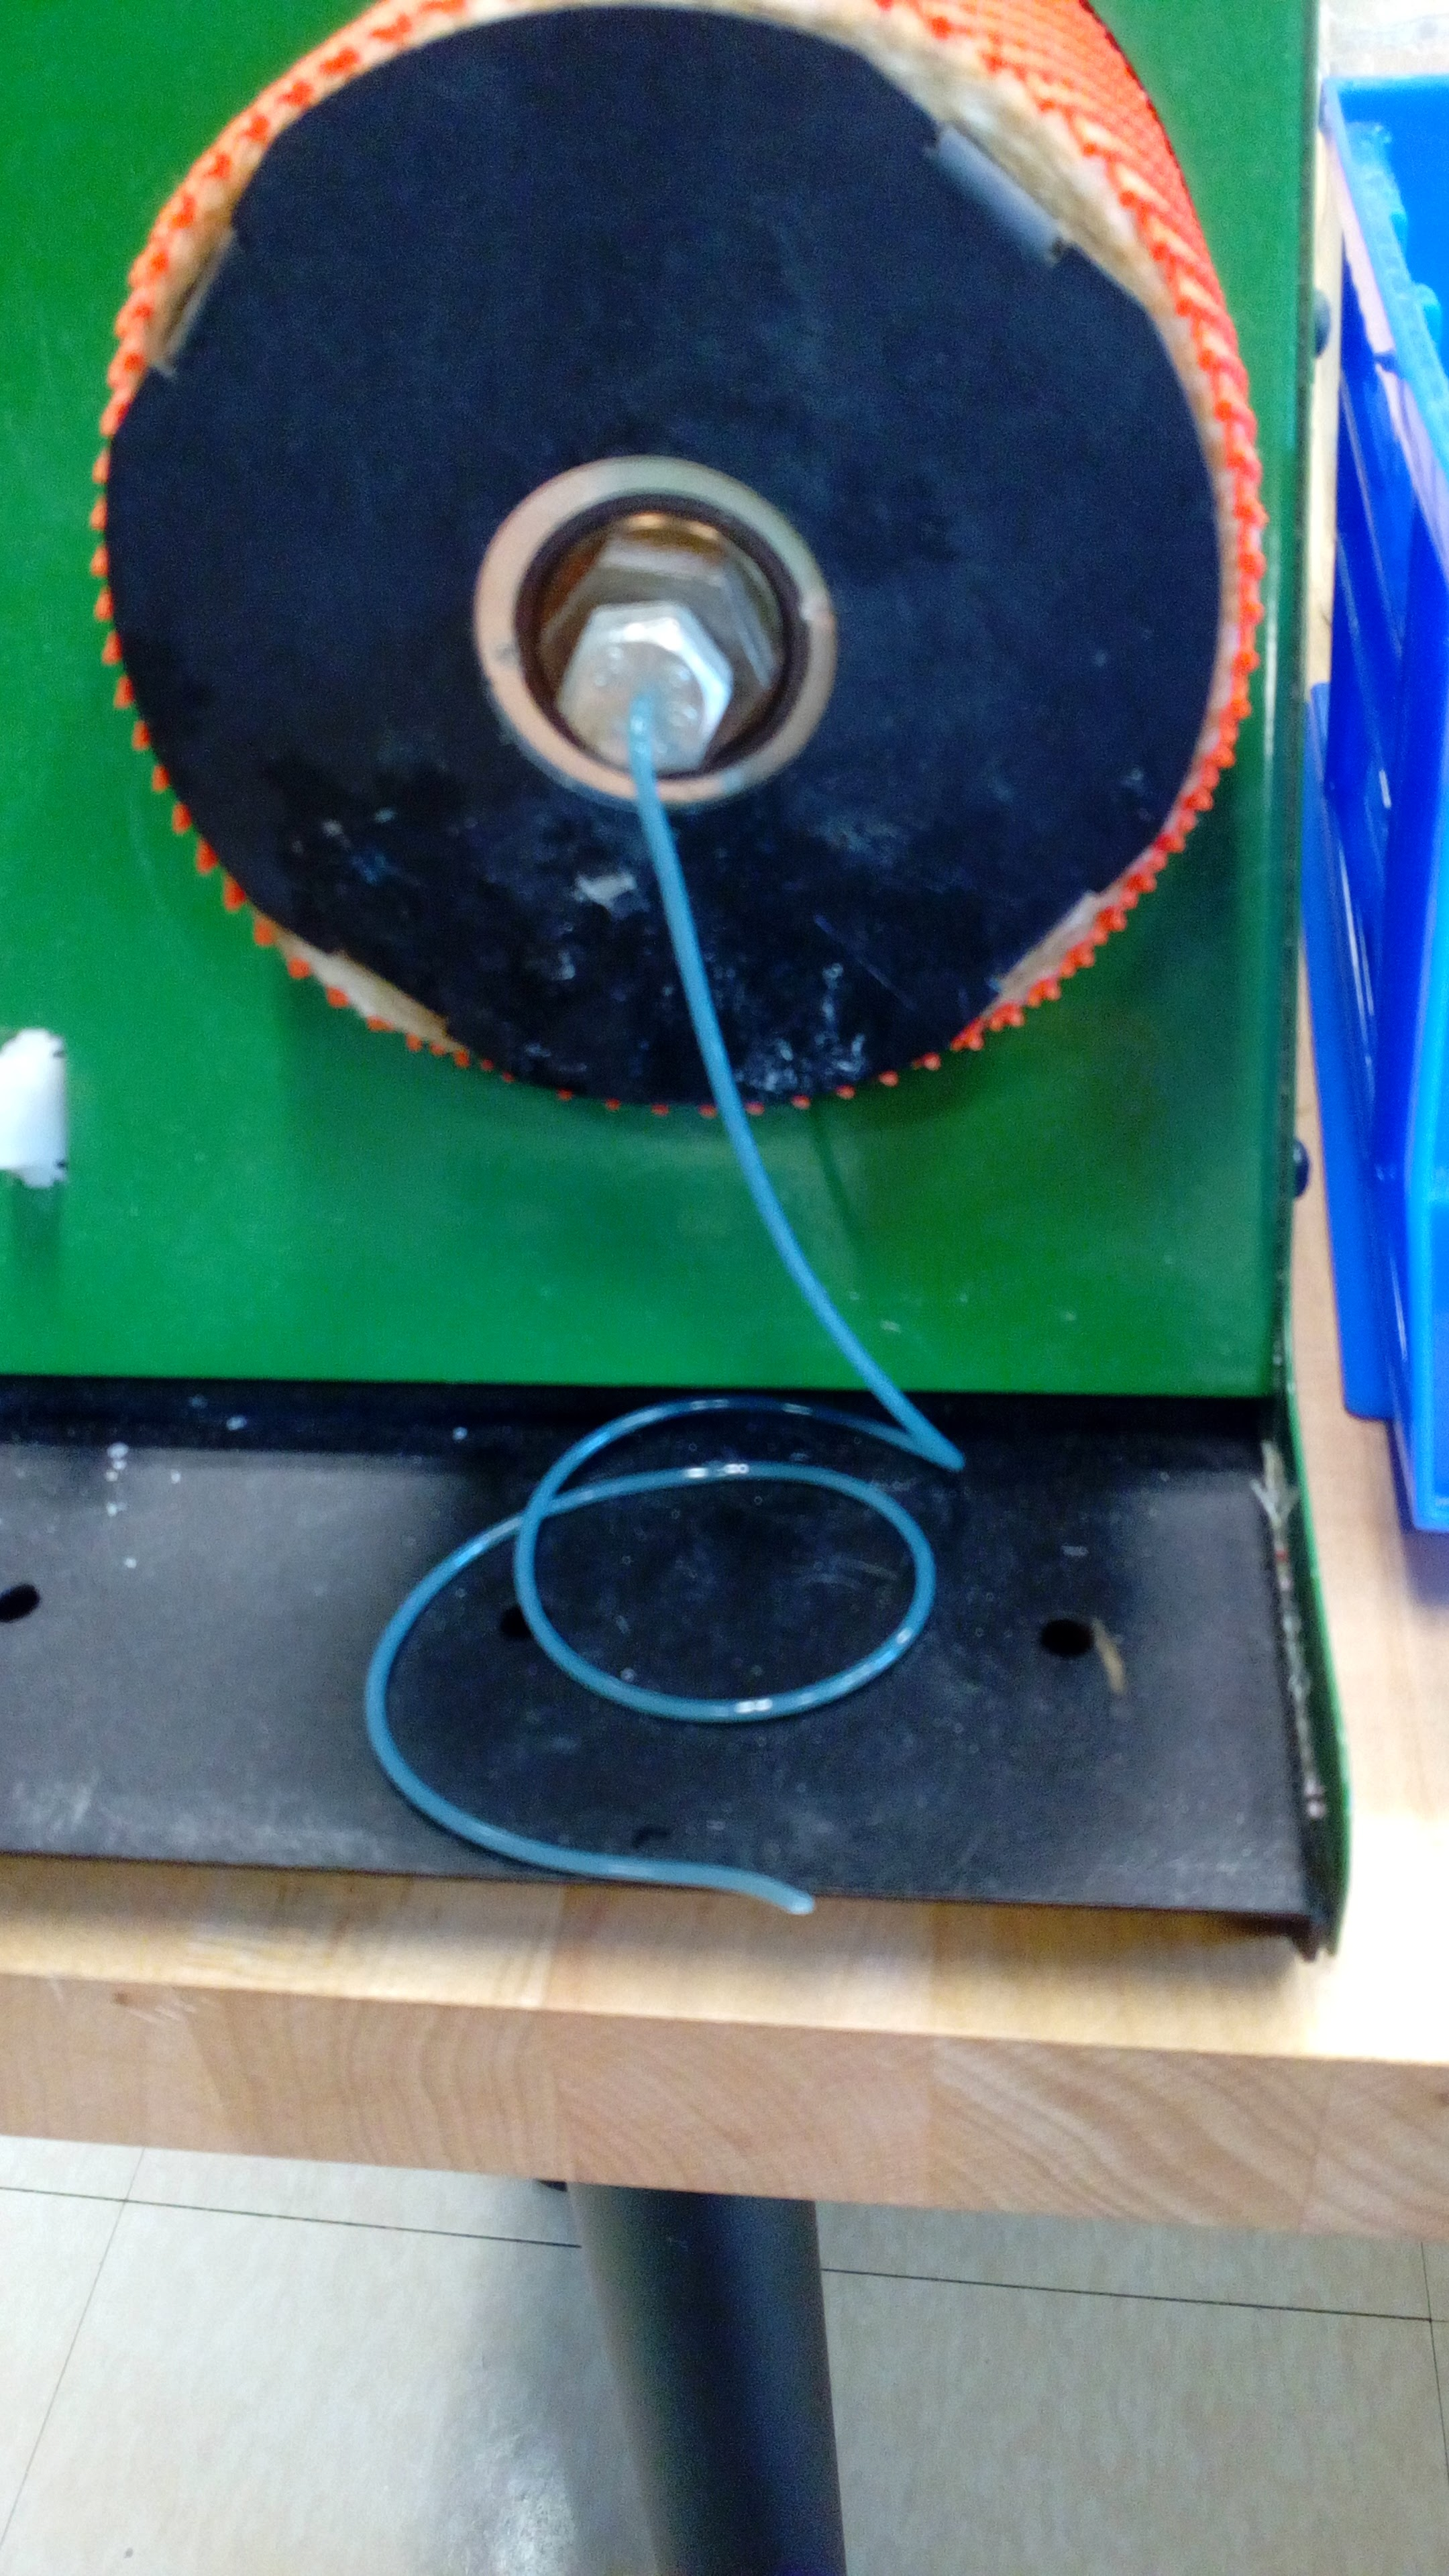
\includegraphics[width=0.5\hsize]{art/IMG_20160801_121017.jpg}
\caption{\label{fig:art_2}  }
\end{figure}

\begin{figure}[h!]
\centering
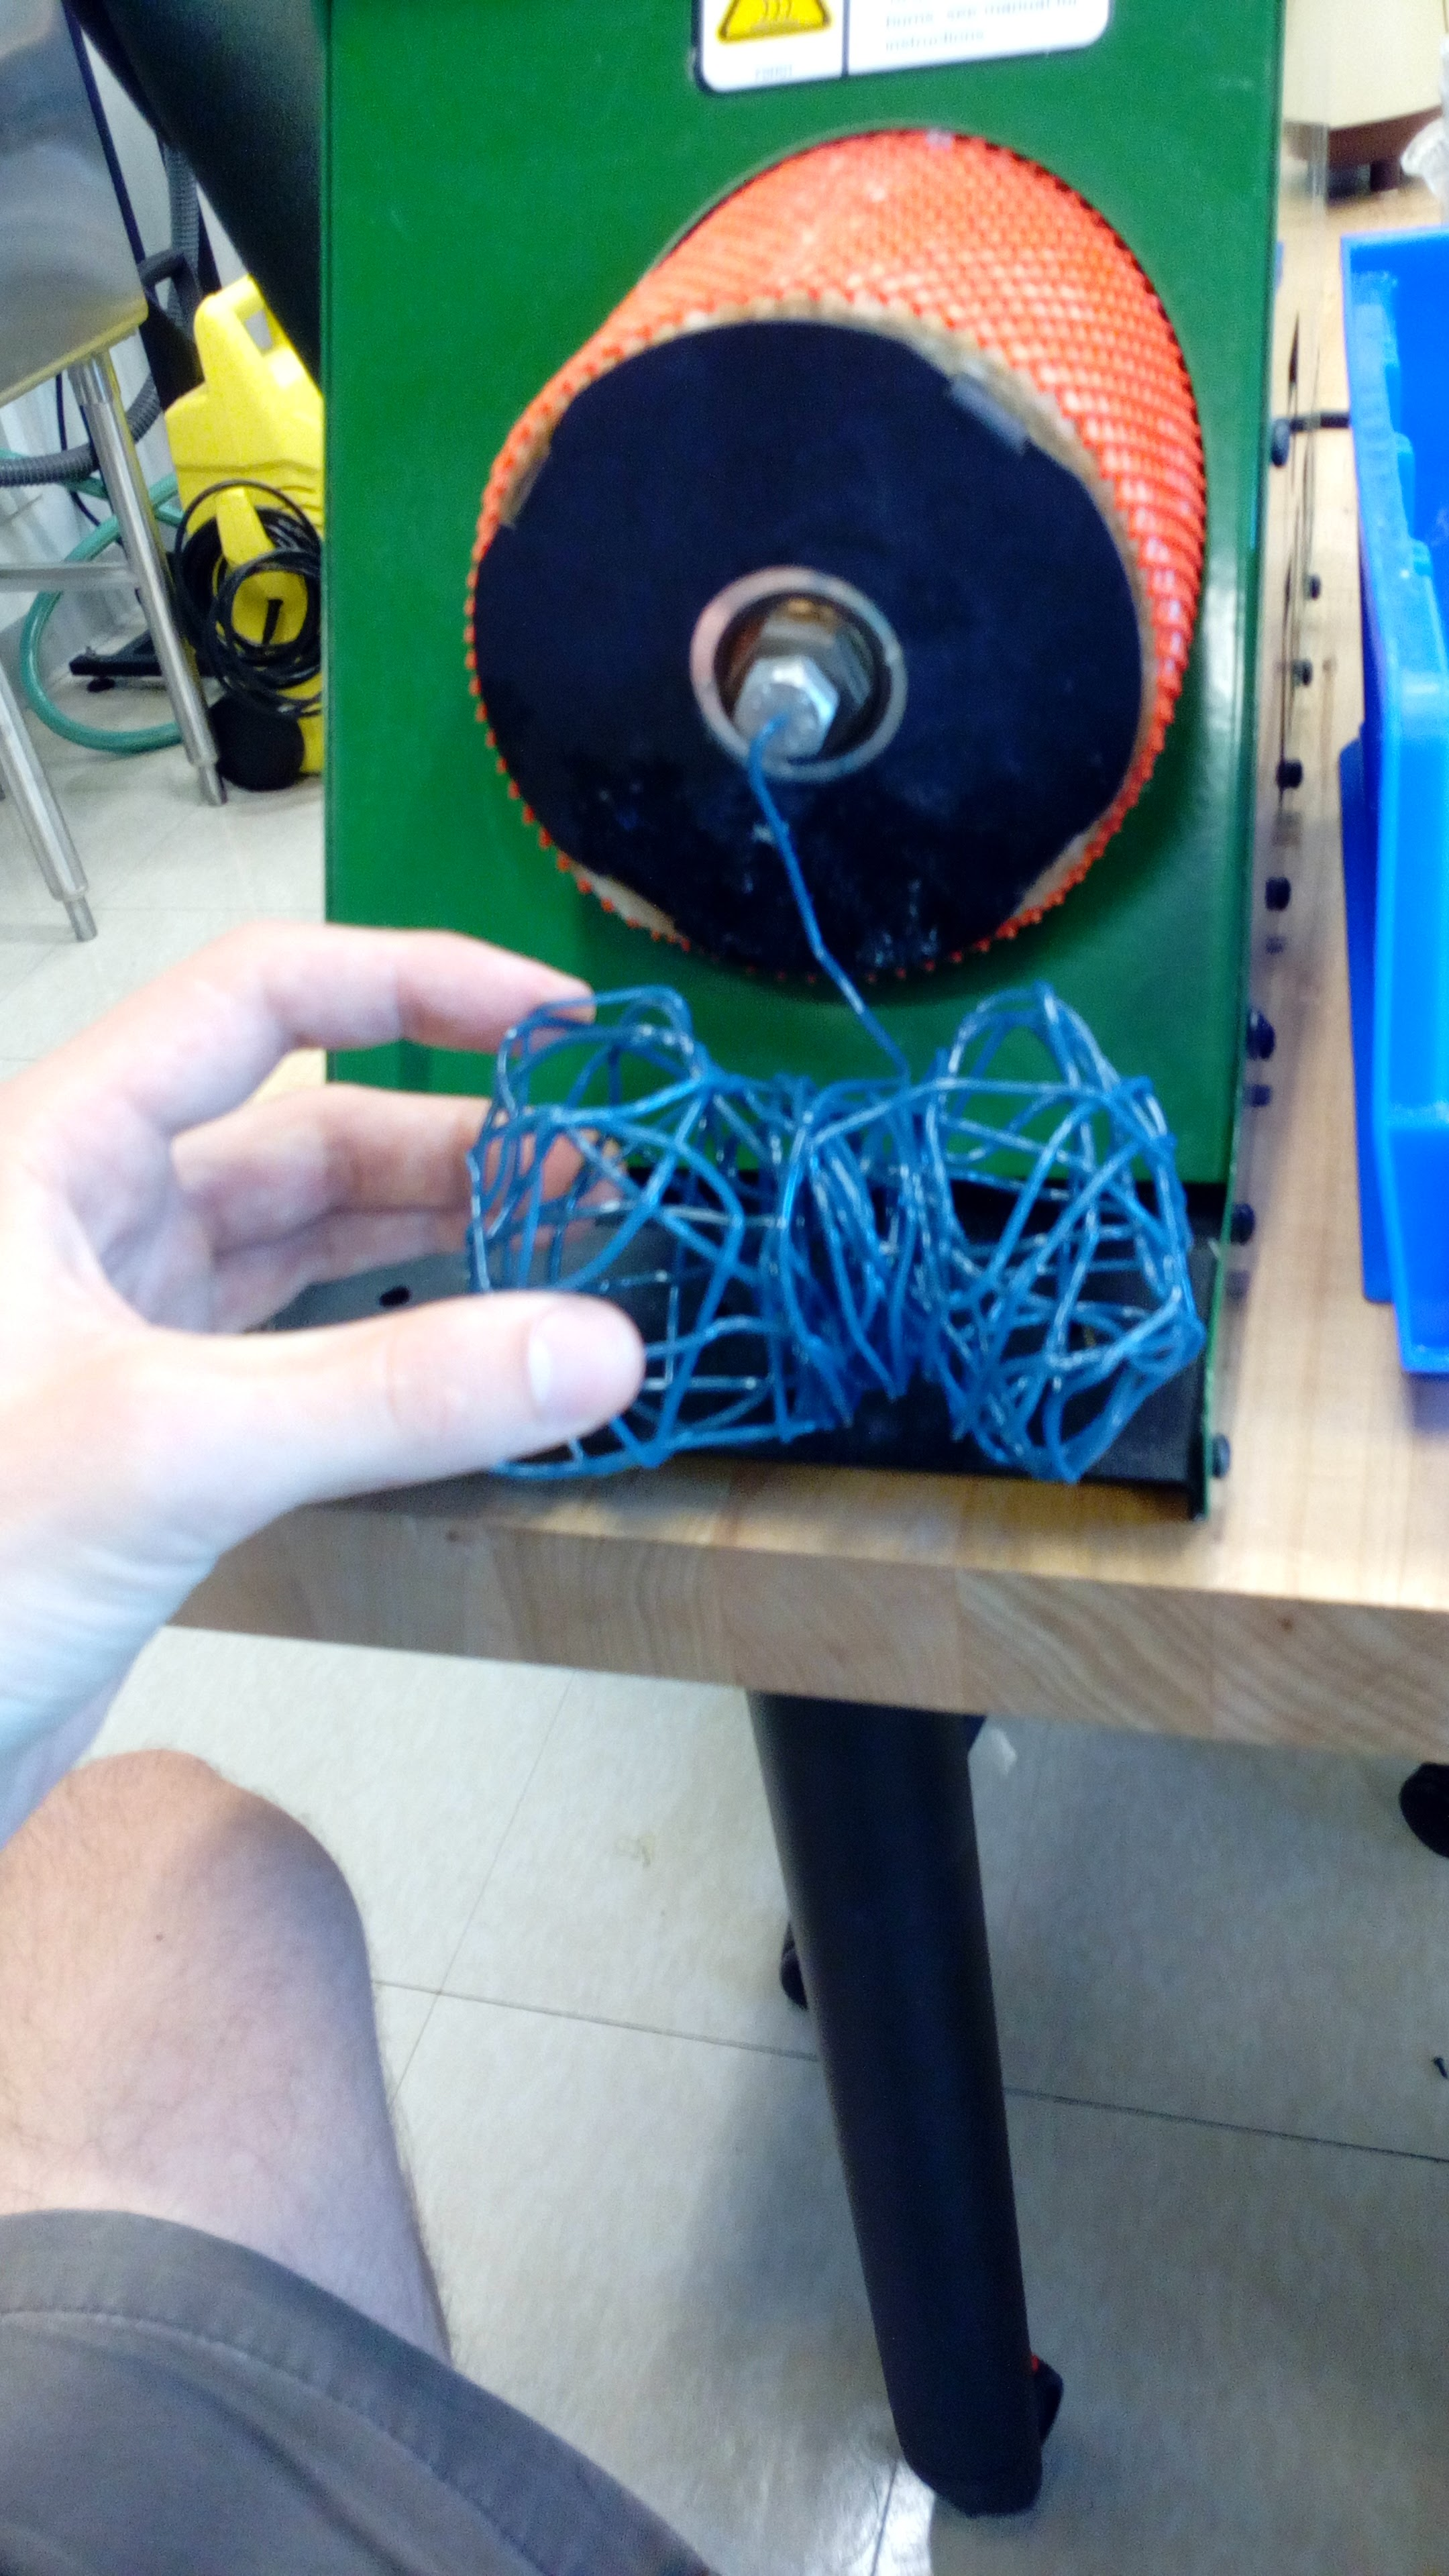
\includegraphics[width=0.5\hsize]{art/IMG_20160801_115125.jpg}
\caption{\label{fig:art_1}  }
\end{figure}



\begin{figure}[h!]
\centering
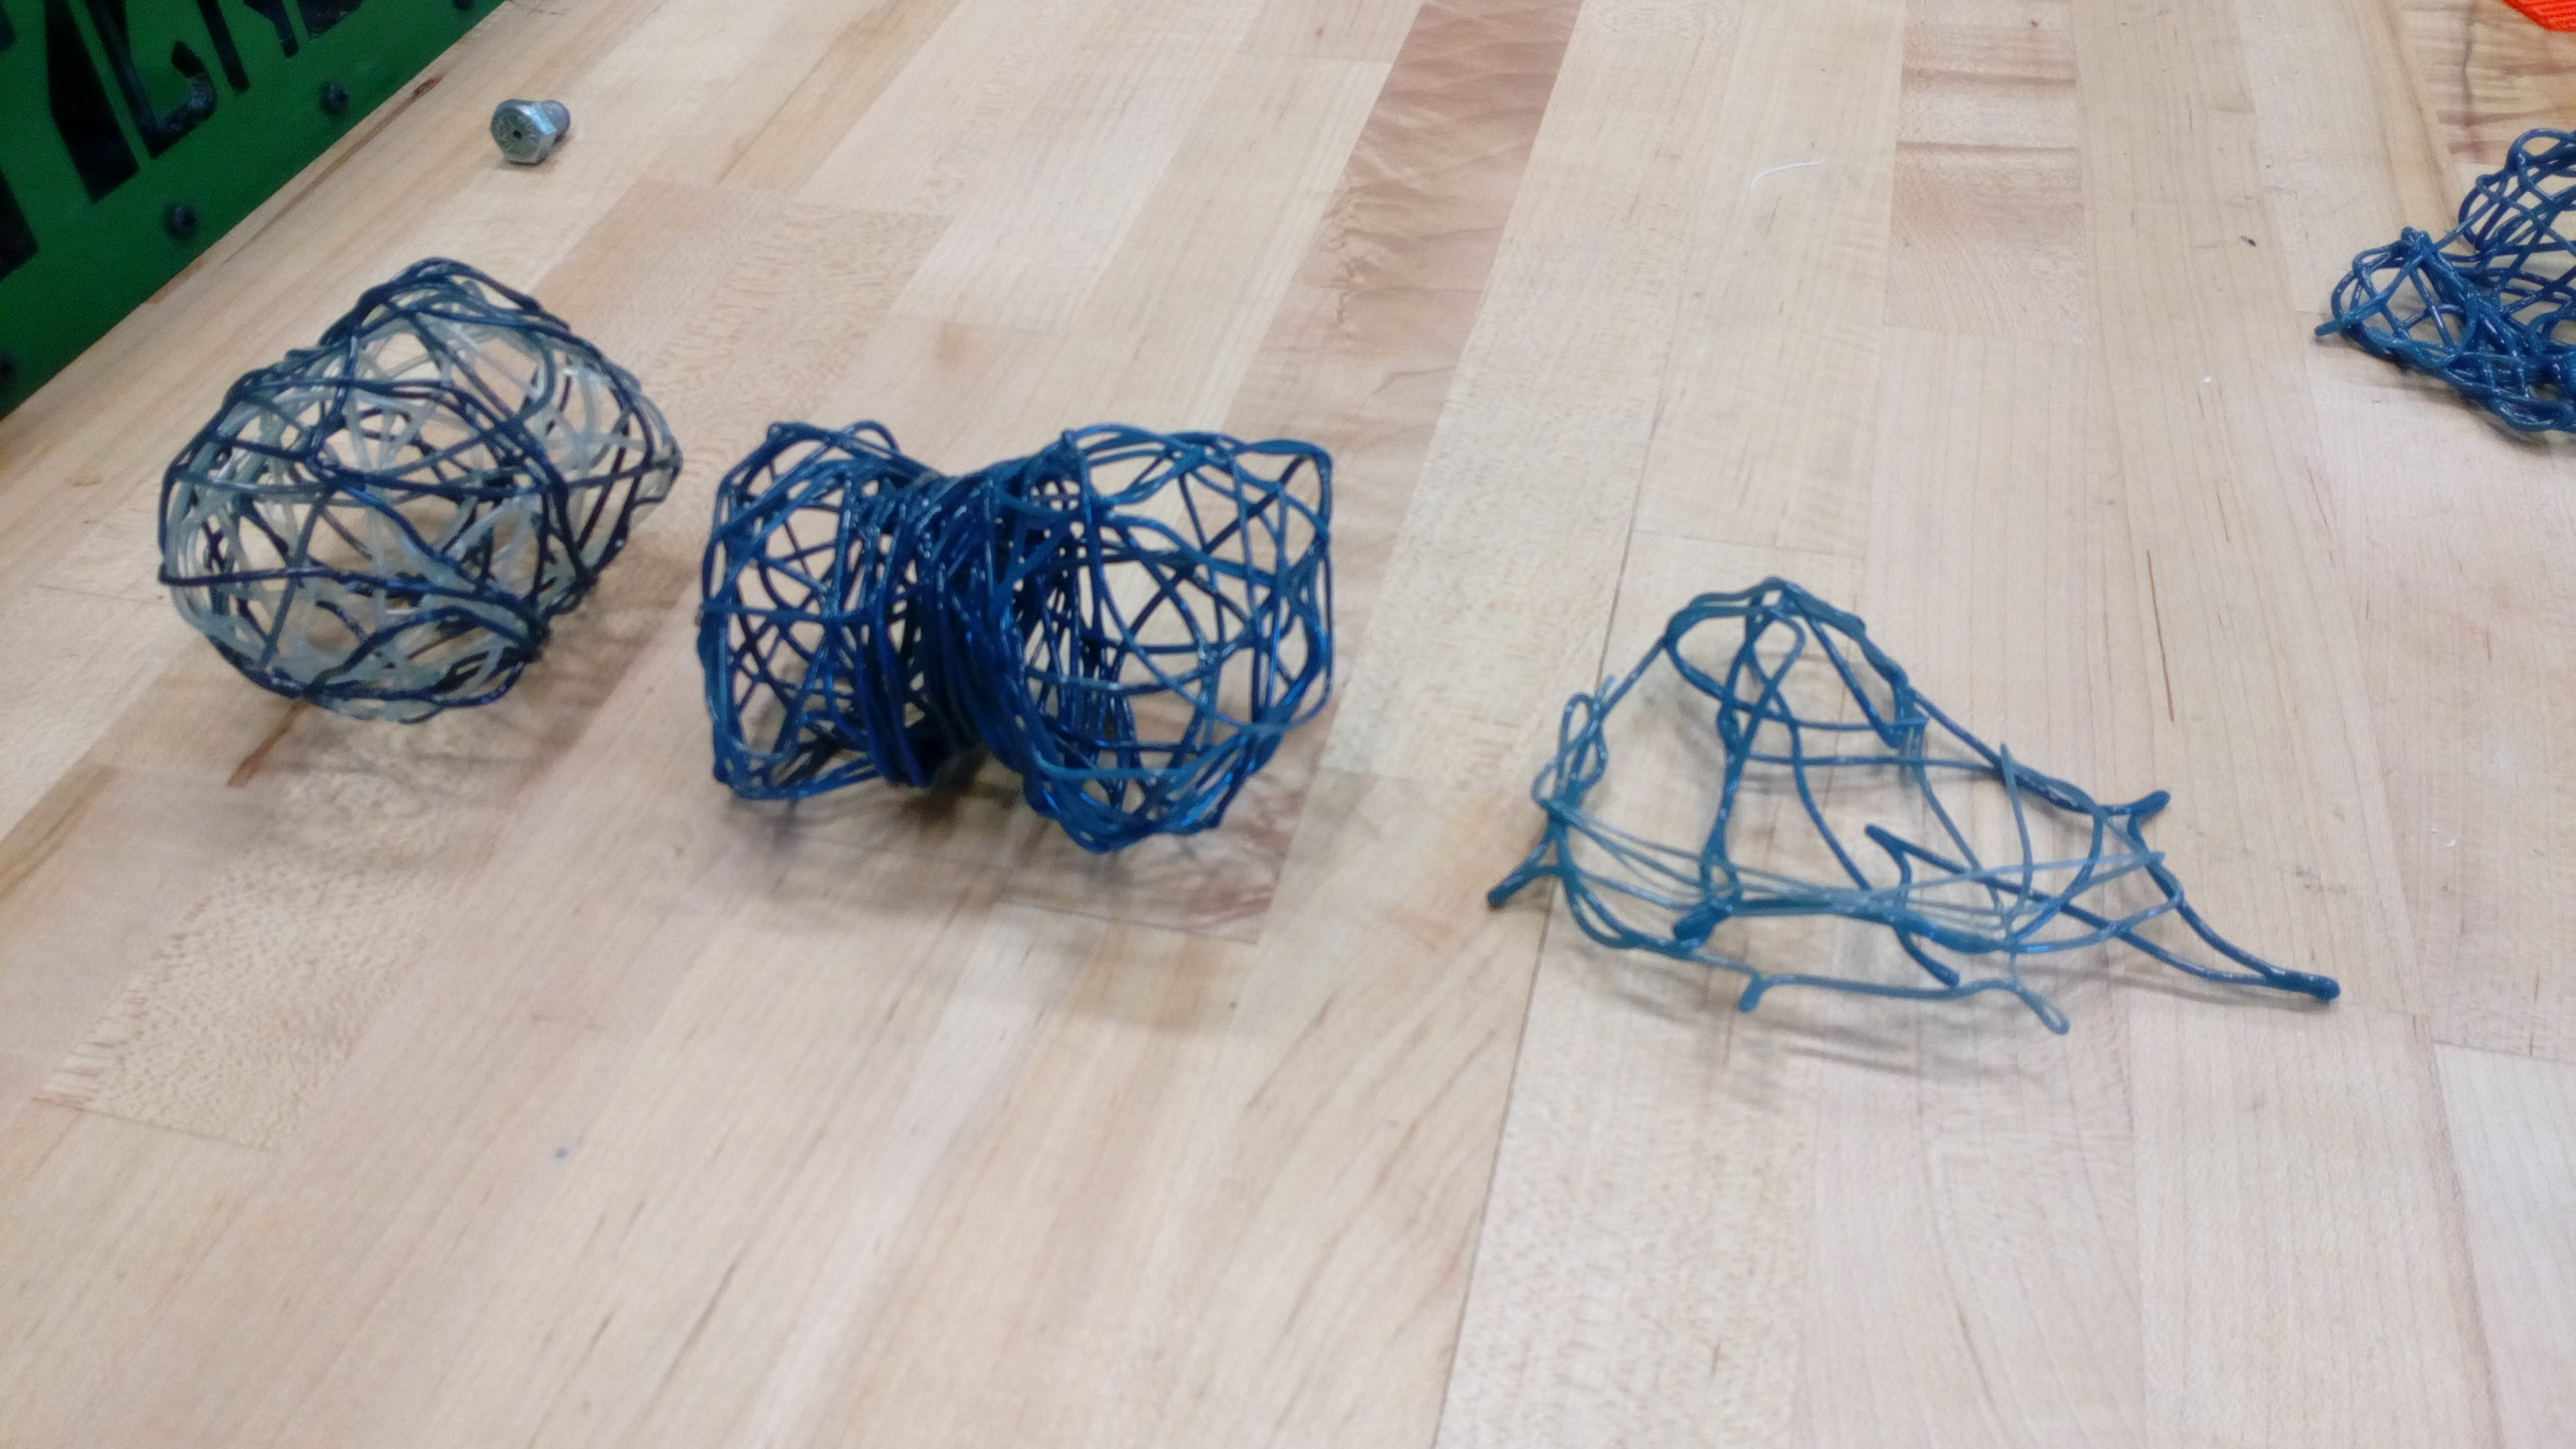
\includegraphics[width=\hsize]{art/IMG_20160801_121232.jpg}
\caption{\label{fig:art_3}  }
\end{figure}

\begin{figure}[h!]
\centering
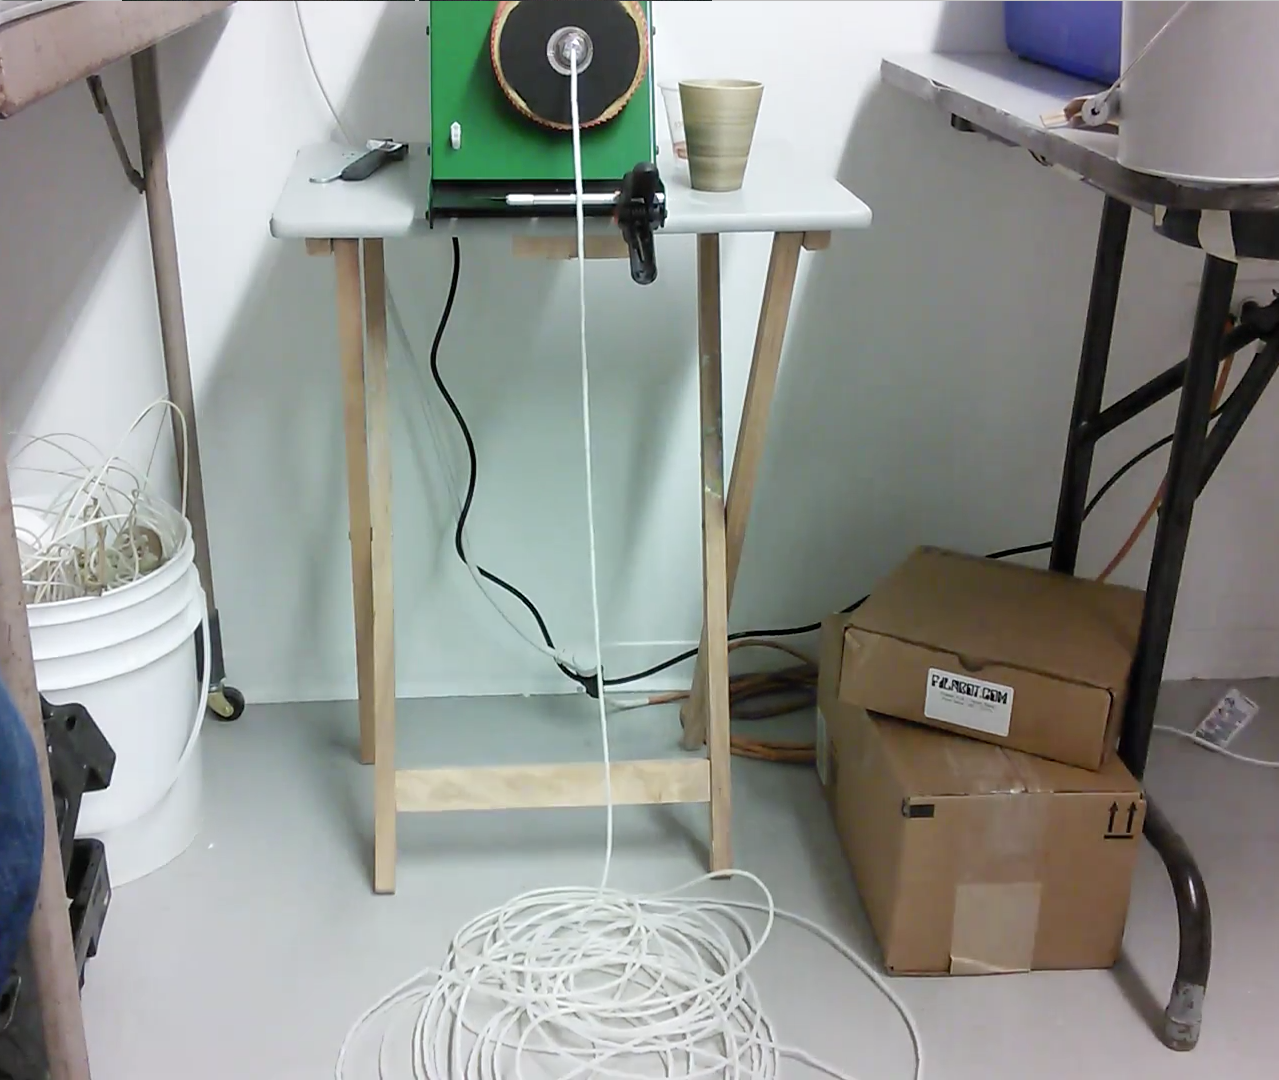
\includegraphics[width=\hsize]{art/extruding.png}
\caption{\label{fig:art_2}  }
\end{figure}

\begin{figure}[h!]
\centering
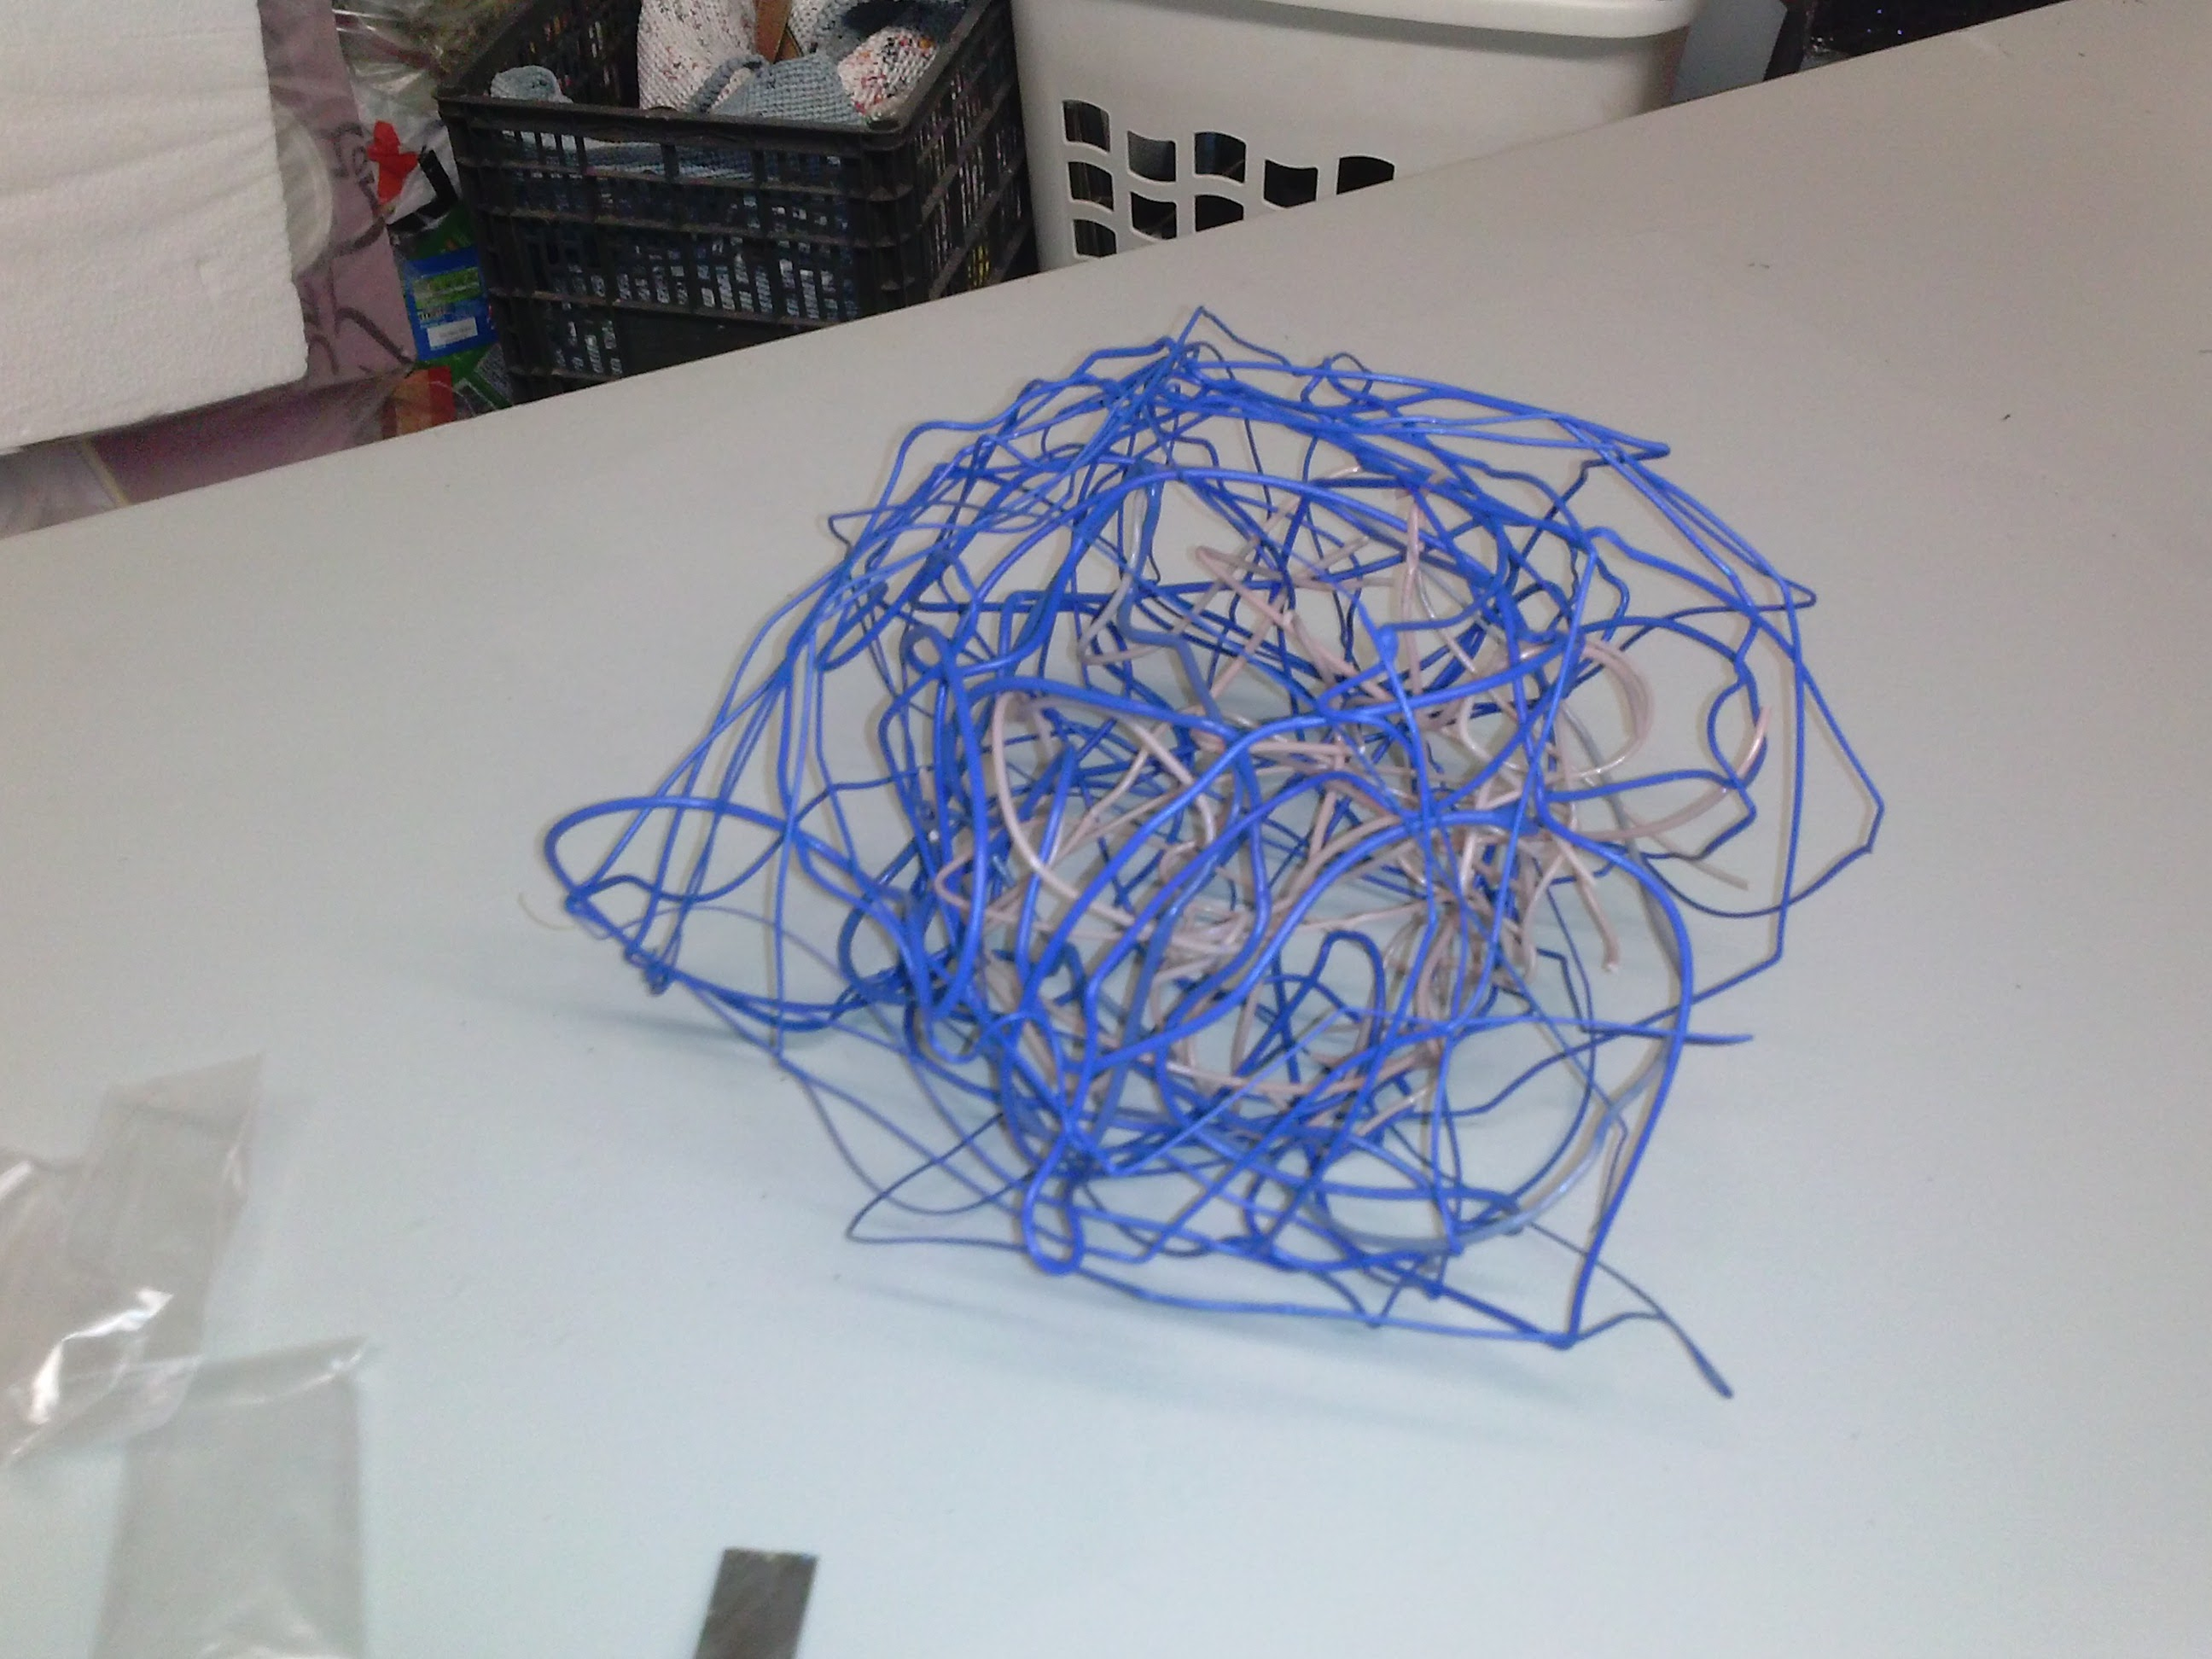
\includegraphics[width=\hsize]{art/CAM00454.jpg}
\caption{\label{fig:art_1}  }
\end{figure}



\begin{figure}[h!]
\centering
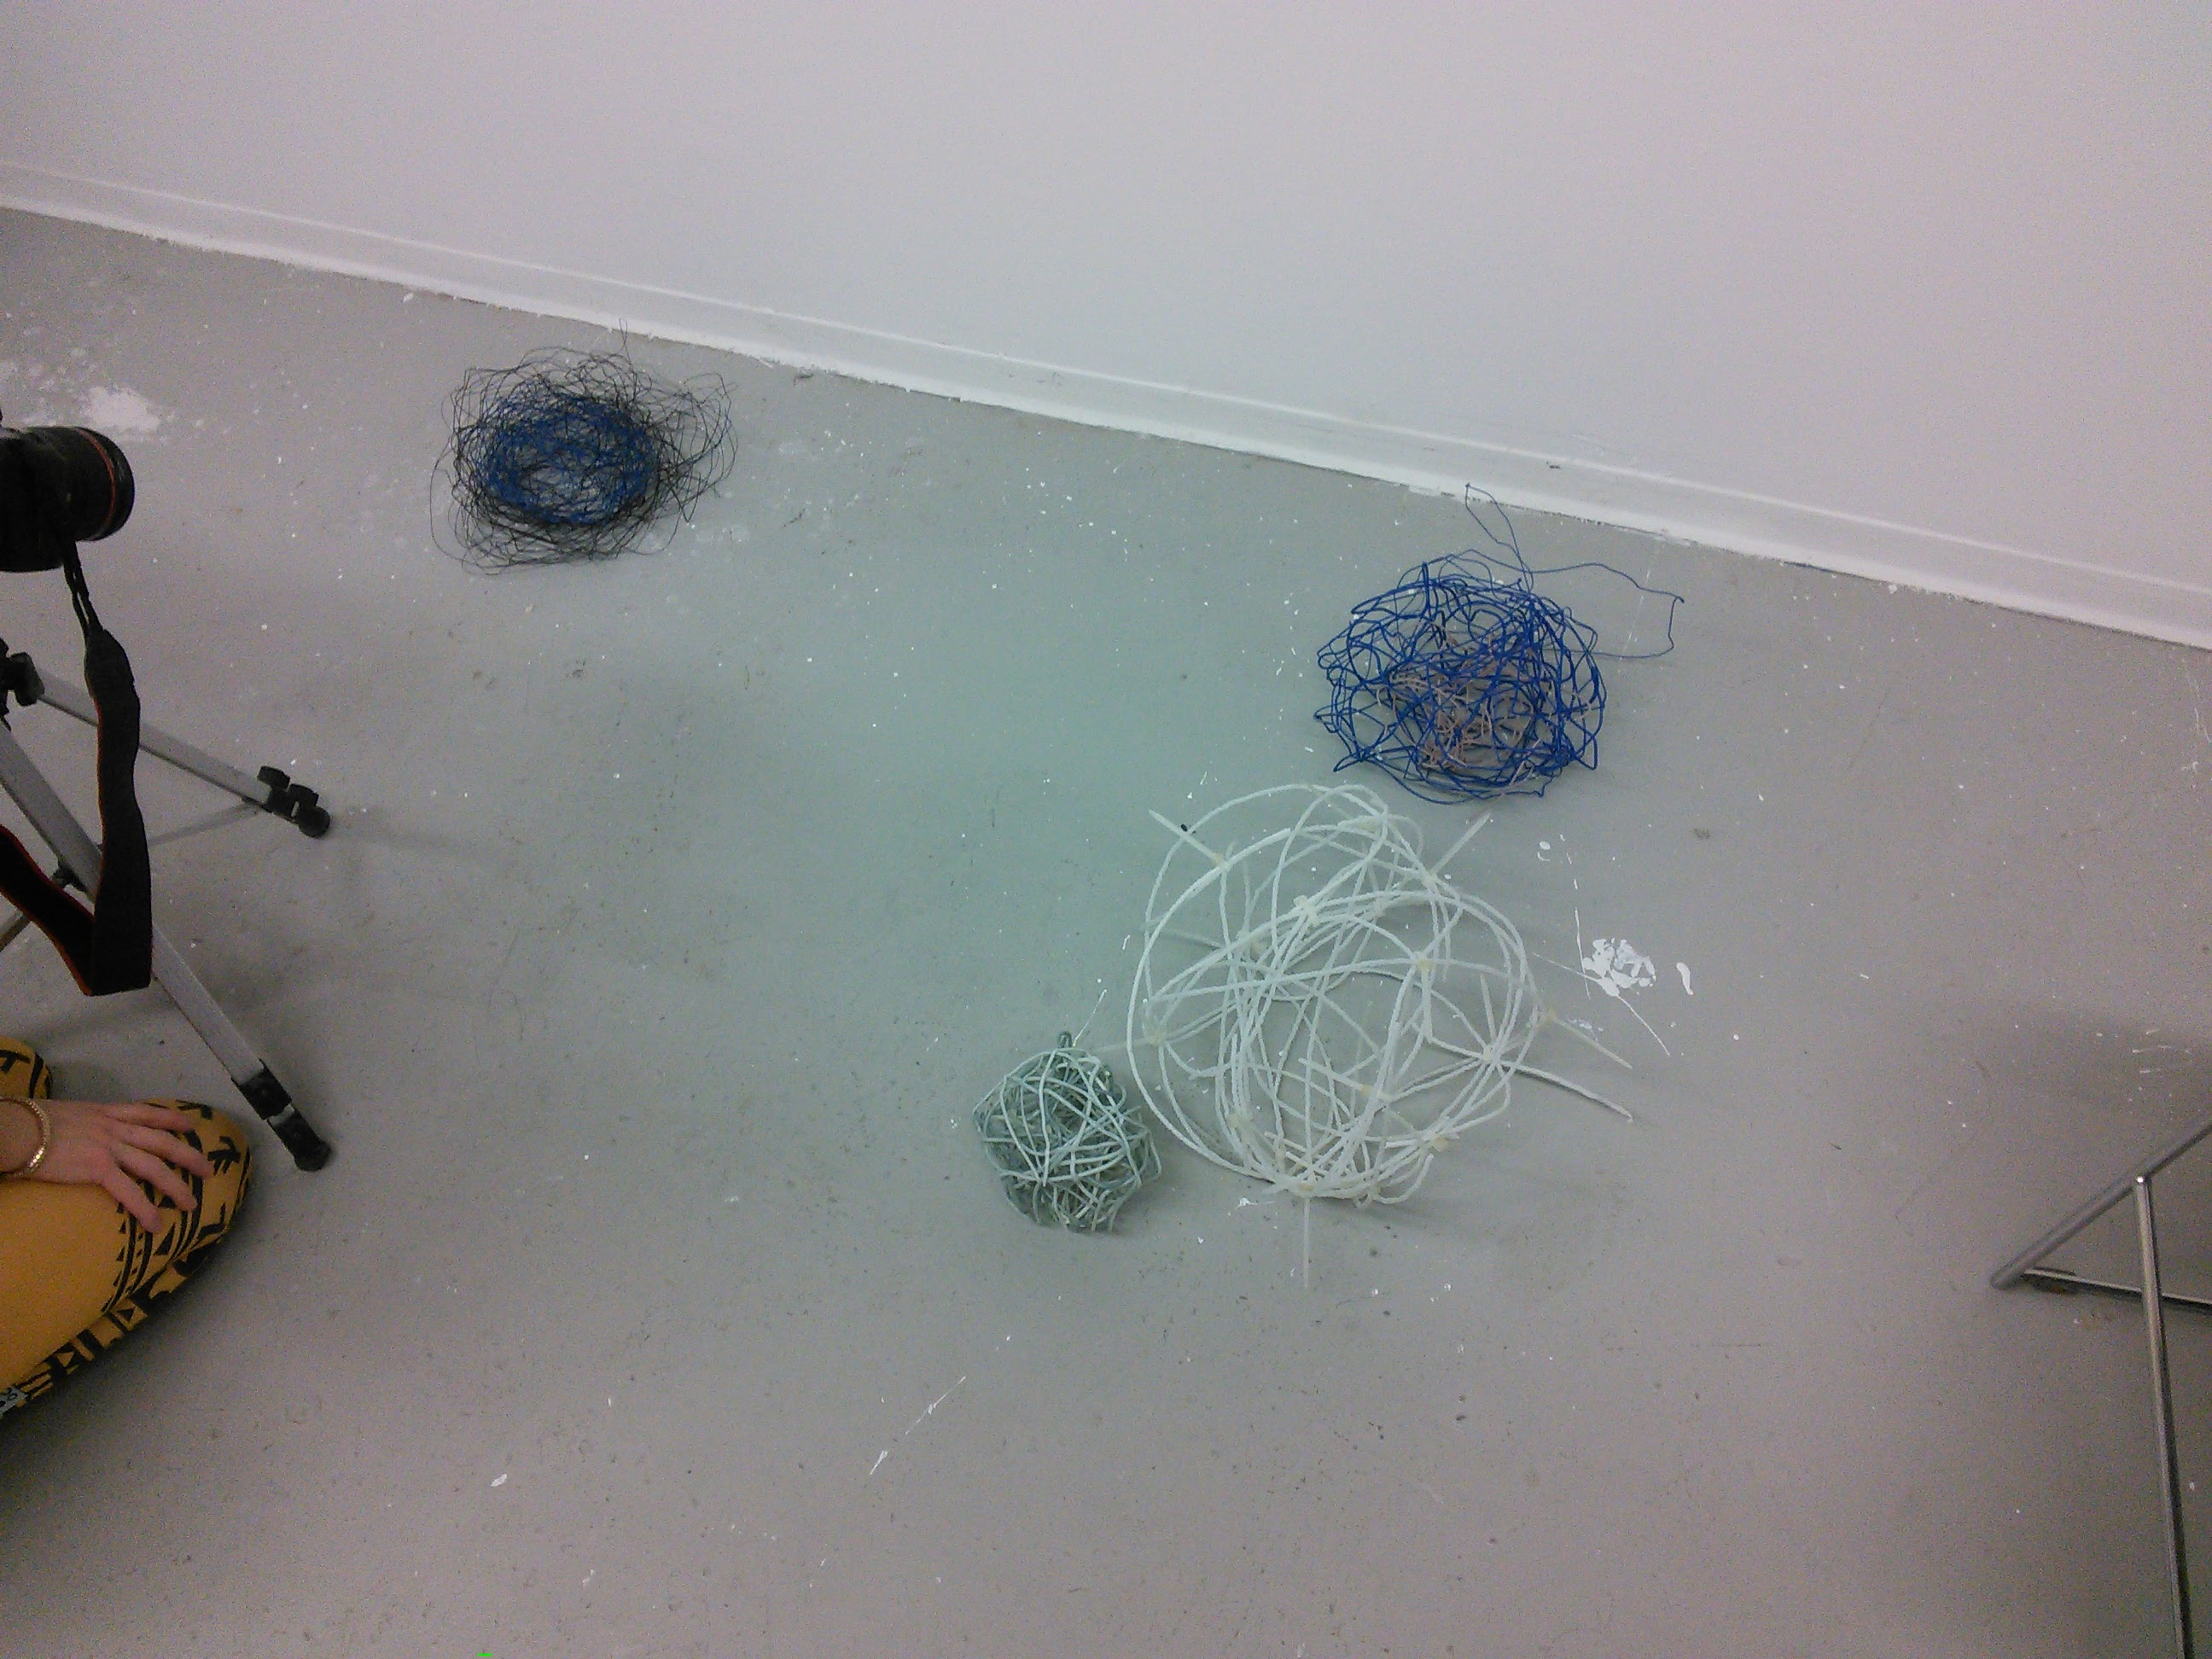
\includegraphics[width=\hsize]{art/IMG_20160205_113249.jpg}
\caption{\label{fig:art_3}  }
\end{figure}